% !TeX spellcheck = en_US
% !TeX encoding = UTF-8
% !TeX root = ../document.tex

\newcommand{\TSprime}{\ensuremath{\TS'}\xspace}
\newcommand{\ntrue}{\ensuremath{n_\text{true}}\xspace}
\newcommand{\nexp}{\ensuremath{n_\text{exp}}\xspace}
\newcommand{\nobs}{\ensuremath{n_\text{obs}}\xspace}
\newcommand{\sigmatrue}{\ensuremath{\sigma_\text{true}}\xspace}
\newcommand{\sigmaexp}{\ensuremath{\sigma_\text{exp}}\xspace}

\chapter{Additional Studies}
\section{Coverage Analysis}
In this chapter, we will show that the test statistic \TS introduced in \fref{sec:test_statistic} can be directly interpreted as $p$-value: $p = \TS$. We will refer to the definition and requirements of a $p$-value and show that \TS sufficiently fulfills those requirements.
Additionally, we will repeat the analysis with \TSprime, using a normal prior (as used in previous \acs{MUSiC} theses) instead of the log-normal term in \TS and compare the results.

A $p$-value is an indicator for the significance of a deviation, where a smaller $p$-value corresponds to a higher significance. The $p$-value of a result is compared to a significance threshold $\alpha$, which is fixed before the statistical analysis. If the observed $p$-value is smaller than $\alpha$, the null hypothesis is rejected. In our case, rejection of the null hypothesis corresponds to falsification of the \acl{SM} and thus the discovery of new physics. 

Both values are constructed in way that the null hypothesis is (incorrectly) rejected by chance with a probability of $\alpha$:
\begin{align}
	\Pr( H_0\:\text{rejected} | H_0 ) &= \alpha \\
    \label{eq:coverage_inequality}
    \Rightarrow \Pr( p < \alpha | H_0 ) &= \alpha
\end{align}
This equation is tested during the \emph{coverage analysis}.

\subsubsection{Procedure}
To test \fref{eq:coverage_inequality}, we construct pseudo experiments based on the null hypothesis $H_0$ and calculate the corresponding $p$-value, in this case \TS or \TSprime. After generating and examining sufficiently many pseudo experiments, we can determine the rate of significant findings and compare them to the claimed significance threshold:
\begin{equation}
	p_\text{true} = \frac{\text{number of pseudo-experiments where $p < \alpha$}}{n_\text{toys}} = \Pr(p < \alpha | H_0)
    \label{eq:coverage}
\end{equation}

The pseudo experiments are based on \acs{MUSiC}'s null hypothesis: 
We assume that there is a constant probability that events end up in a particular region, and thus a constant true mean value \ntrue. 
We also assume that this true mean value is only known up to an expected event yield, \nexp.
The way that \nexp is derived from \ntrue differs between \TS and \TSprime: For \TS, \nexp is drawn from a log-normal probability density, \TSprime  will use a normal distribution instead.

Additionally, the physics process of performing a counting experiment has to be simulated: Here it is assumed that the event yield is caused by independent statistical processes with a fixed probability, thus the observed event yield follows a Poisson distribution around \ntrue.

The way that the assumed uncertainty enters the pseudo experiment also differs between \TS and \TSprime: For \TS, we recalculate the uncertainty after drawing \nexp in order to keep the relative uncertainty constant: $\sigmaexp = \frac{\nexp}{\ntrue} \sigmatrue$. For \TSprime, the absolute uncertainty is kept constant: $\sigmaexp = \sigmatrue$.
This has been argued by \cite[p. 78]{Schmitz:ModelUnspecificSearch}, a more rigorous discussion can be found in \fref{app:coverage_uncertainty}.

In the implementation, each pseudo-experiments begins with drawing \nexp from the probability density around \ntrue. At the same time, \nobs is drawn from a (discrete) Poisson distribution with a mean of \ntrue. From these two values, as well as the uncertainty \sigmaexp, \TS (or \TSprime) is calculated.

This process is repeated for $n_\text{toys}$ pseudo-experiments. An estimation for the true $p$ value is afterwards calculated using \fref{eq:coverage}, which yields the left hand side of \fref{eq:coverage_inequality}.

In order to state the so called "coverage value" for the tuple (\ntrue, \sigmatrue), both sides of  \fref{eq:coverage_inequality} are translated to $Z$-scores (see \fref{app:z_score}), resulting in $Z_\text{true} = Z(p_\text{true})$ representing the observed and $Z_\text{claim} = Z(\alpha)$ representing the claimed rate ob significant results.
The coverage is finally reported as
\begin{equation}
    \label{eq:coverage_value}
	\text{coverage} = Z_\text{true} - Z_\text{claim}.
\end{equation}
%or alternatively as 
%\begin{equation}
%    \text{coverage}' = \log_{10} %\left(\frac{p_\text{true}}{p_\text{claim}}\right)
%\end{equation}

\subsubsection{Interpretation of Results}
Three different result cases can arise, depending on the coverage value in \fref{eq:coverage_value}:
\begin{enumerate}
	\item $\text{coverage} = 0 \Leftrightarrow \Pr( H_0 \text{ rejected} | H_0 ) = \alpha$: This is the ideal case. It indicates the $p$-value performs according to its definition.
	\item $\text{coverage} < 0 \Leftrightarrow \Pr( H_0 \text{ rejected} | H_0 ) > \alpha$: The background hypothesis is rejected more often than with a probability of $\alpha$. This case is called "undercoverage" and corresponds to "liberal" behavior. The $p$-value overestimates the significance of deviations.
	\item $\text{coverage} > 0 \Leftrightarrow \Pr( H_0 \text{ rejected} | H_0 ) < \alpha$: The background hypothesis is not rejected in some cases where it should have been rejected. This effect is called "overcoverage" and corresponds to "conservative" behavior where the $p$-value underestimates the significance of deviations.
\end{enumerate}	

\subsubsection{Our Results}
Since the MUSiC $p$-value is required to cover a large range of possible \ntrue and relative uncertainty $\sigmatrue / \ntrue$ values, the coverage is evaluated on a two dimensional grid in this parameter space.
The computed results can be found in \fref{fig:coverage}.

\begin{figure}
    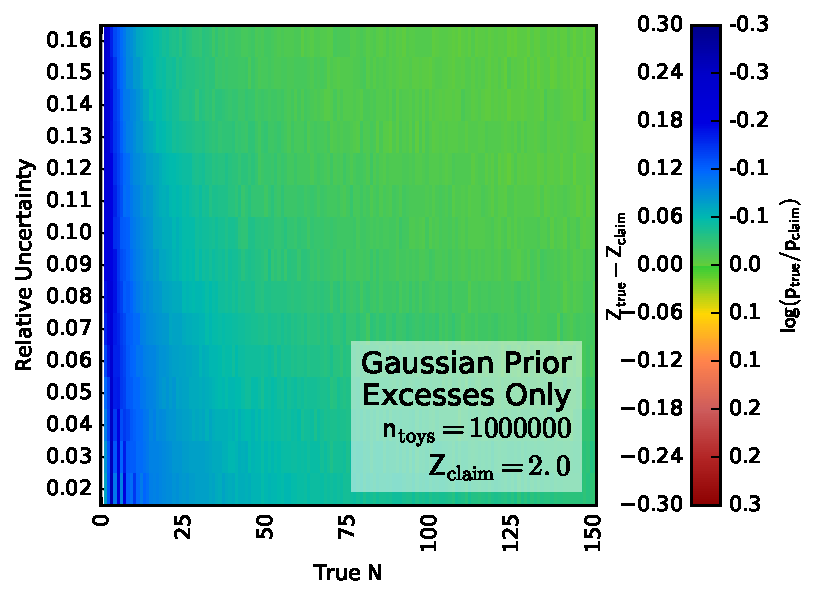
\includegraphics[width=\textwidth]{coverage/coverage_excess_normal_schmitz}
    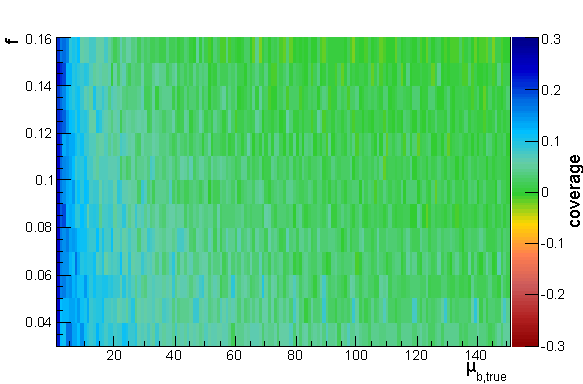
\includegraphics[width=\textwidth]{schmitz_coverage}
    \caption{Comparison of our results (top) with \cite{Schmitz:ModelUnspecificSearch} (bottom). The test settings as well as plotting options have been chosen to match. From visual inspection one can deduce that the results are very similar, which allows us to directly compare results from our implementation with the earlier thesis.}
    \label{fig:coverage_schmitz}
\end{figure}

\begin{figure}
    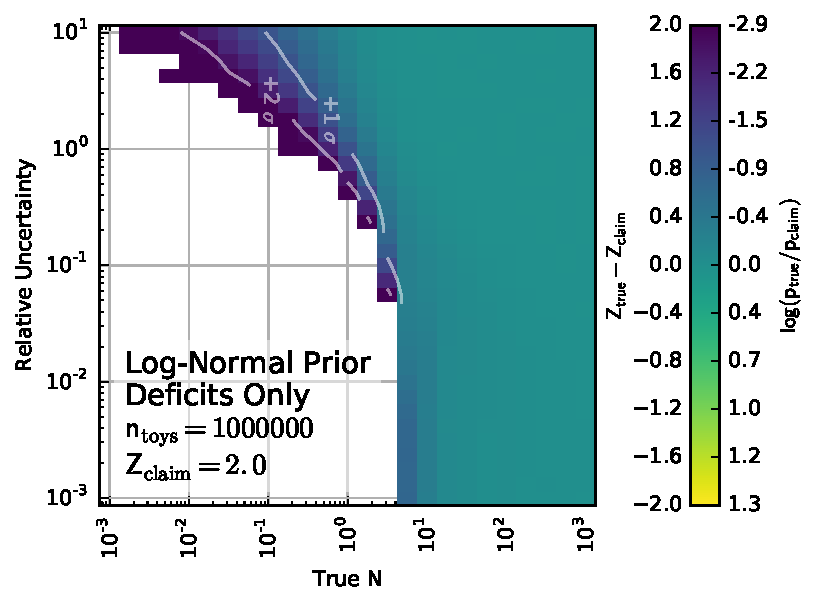
\includegraphics[width=\textwidth]{coverage/coverage_deficit_lognormal_log}
    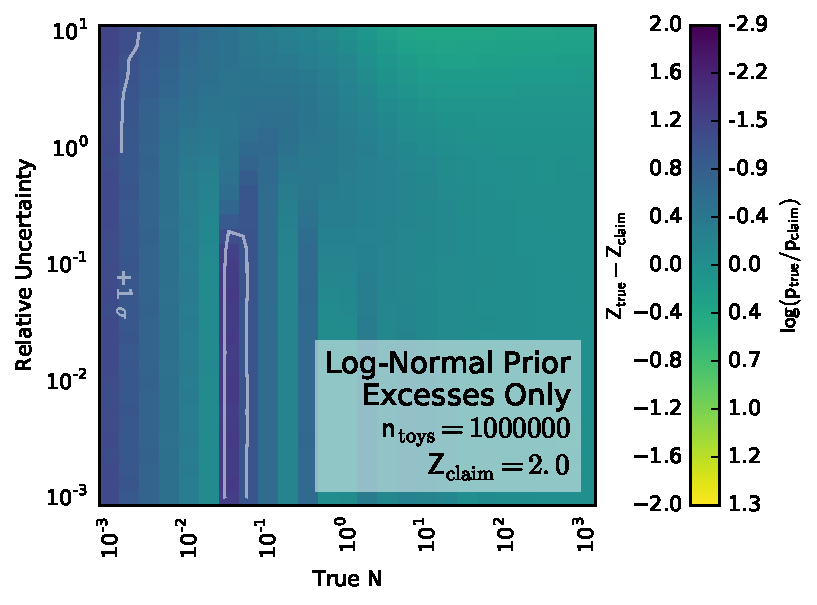
\includegraphics[width=\textwidth]{coverage/coverage_excess_lognormal_log}
    \caption{Results of the coverage analysis.}
    \label{fig:coverage}
\end{figure}

\begin{figure}
    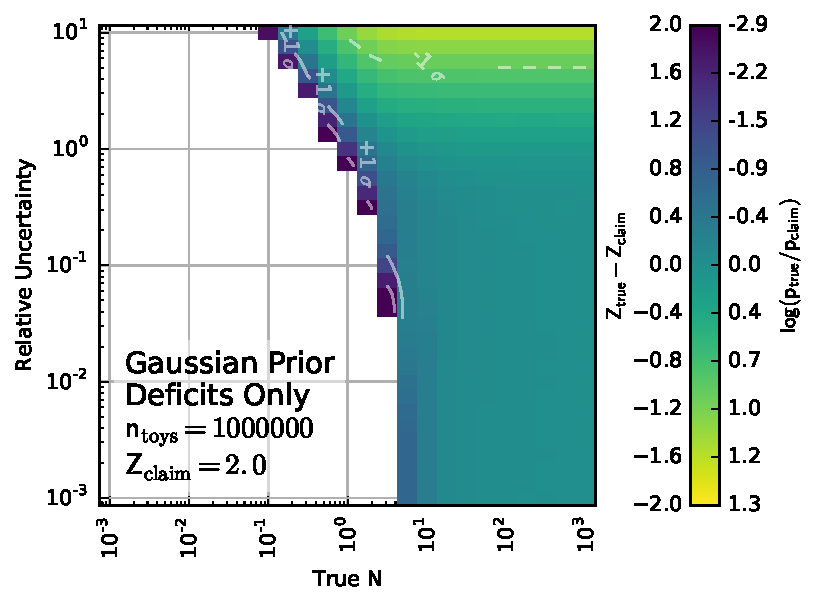
\includegraphics[width=\textwidth]{coverage/coverage_deficit_normal_log}
    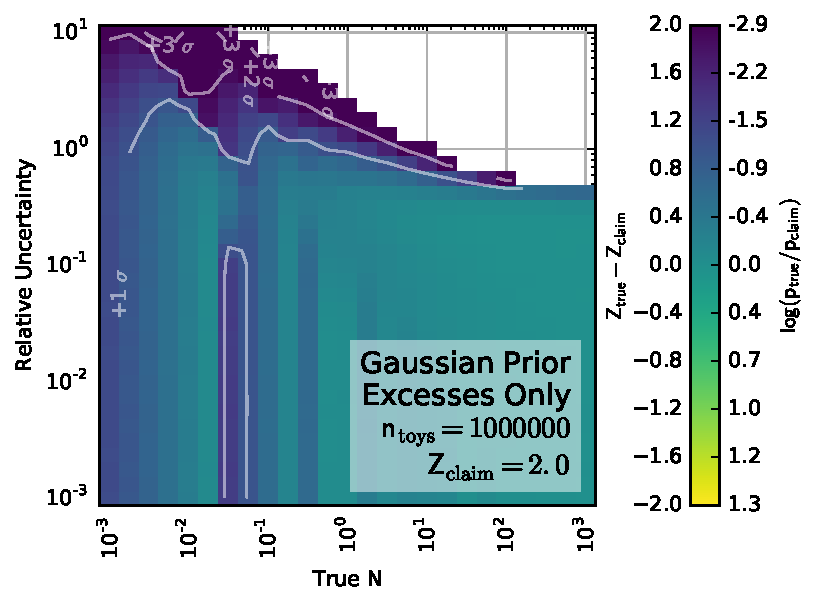
\includegraphics[width=\textwidth]{coverage/coverage_excess_normal_log}
    \caption{Results of the coverage analysis.}
    \label{fig:coverage2}
\end{figure}


\section{Log-Normal $p$-Value}


\section{A Global $p$-Value}
\newcommand{\TSphat}{\ensuremath{T}\xspace}

The \ptilde distribution provides the ability to register less significant deviations in many classes by looking at the central part of the distribution. However, this manual method is only qualitative. We will now introduce a possible extension to the analysis which provides a quantitative method of combining the \ptilde values of all classes.

This not only allows us to draw conclusions about the presence of new physics in our observed data set, but also to quantify \ac{MUSiC}'s sensitivity for simulations of known benchmark models. Furthermore, an automated analysis can be used as regression test to decide whether future modifications to the analysis improve its sensitivity.

As before, the desired output for such a global method is a $p$-value which can then be compared to a significance threshold $\alpha$.
As input, the algorithm takes the look-elsewhere-corrected \ptilde values of all classes. In the case of \ac{MC} simulation, either for \ac{SM} or signal studies, such a set of \ptilde values can be provided for each pseudo experiment round, for observed data we only obtain one list (one value for each class).

The algorithm for the \ac{SM} distribution goes as follows: For each pseudo experiment round, the distribution of \ptilde values (of call classes) is compared to a reference distribution using a statistical test. The test outputs a scalar result \TSphat, where a larger value indicates a larger deviation from the reference distribution. \TSphat is then noted in a separate set, which eventually contains one test statistic value for each pseudo experiment round.
For observed data, the test statistic is calculated for the (only) set of \ptilde-values, resulting in $\TSphat_\text{data}$.

Finally, the resulting \phat value is defined as the rate of pseudo-rounds where $\TSphat > \TSphat_\text{data}$, similar to \ptilde before. This way, full coverage of \phat is guaranteed by definition.

For the quantification of sensitivity, the \emph{test power} $\beta$ for a given signal is calculated. The test power describes the probability that the \ac{SM} null hypothesis is (correctly) rejected if new physics are present in the data set. 
The \ac{SM}-step is applied as described above. \phat is then calculated for each signal pseudo experiment round, resulting in multiple $\TSphat_\text{signal}$ values. After agreeing on a significance threshold $\alpha$, $\beta$ is the rate of significant \TSphat values.

\todo{Problem mit p=1-Klassen erklären (siehe ptilde-distribution)}
%problems: uniform reference vs SM-reference, binning (chi2), possibility of infinite p=1 classes (solution: low-stats treatment + cut at p<0.95)

So far, the choice of statistical test and reference distribution is not specified. In the following, multiple options are discussed. The distribution of \ptilde values under investigation is denoted as $f(\ptilde)$, the reference distribution is $g(\ptilde)$. The cumulative distribution functions are $F(\ptilde)$ and $G(\ptilde)$ respectively. 

\begin{itemize}
    \item $\chi^2$-Test: This test is used to compare two binned distributions. For each bin $i'$, the difference between reference $g'_i$ and comparison $f_i$ is evaluated.
    \begin{equation}
        \TSphat = \frac{\chi^2}{\text{ndof}} = \frac{1}{\text{number of bins}} \sum_i^{\text{bins}} \frac{\left(f'_i - g'_i\right)^2}{g'_i}
    \end{equation}
    A disadvantage of this method is that binning discards information. Additionally, the method works best for large number of event classes.
    
    \item Kolmogorov-Smirnov: This test does not require binning. It compares the cumulative distribution functions of reference and comparison. The maximal distance between $F$ and $G$ is \TSphat.
    \begin{equation}
        \TSphat = \sup_x \abs{F(x) - G(x)}
    \end{equation}
    A disadvantage of this test statistic is that it is most sensitive to deviations in the center of the distribution. Additionally, only the largest difference is used for the result, instead of accumulating the difference.
    
    \item Cramér-von-Mises: The Cramér-von-Mises test statistic consists of the integral over the quadratic difference between the reference and compared cumulative distribution functions:
    \begin{equation}
        \TSphat = n \int_{-\infty}^{\infty}\left(F(x) - G(x)\right)^2 w(x)\, \dd F(x)
    \end{equation}
    where $w(x) = 1$.
    
    \item Anderson-Darling: This test is similar to the Cramér-von-Mises method, but uses $w(x) = \left[G(x)(1 - G(x))\right]^{-1}$ instead, thus giving more weight to both tails of the distribution.
    For this test, there exists a discrete version for comparing with a uniform distribution\cite{Stephens:EDFstatisticsgoodness} and a discrete version for $k$ samples\cite{Scholz:KsampleAnderson}. Both are implemented and used in this analysis.
    
    \item Simple: \TSphat is the ratio of \ptilde values below a critical value, in this case \num{0.1}.
\end{itemize}

A thorough comparison of the afore-mentioned test statistics can be found in \cite{Stephens:EDFstatisticsgoodness}.

For each of the mentioned test statistics, two different reference distributions have been tested: a uniform distribution and the empirical distribution of all \ptilde-values of all pseudo experiment rounds in the \ac{SM} sample.
While the former choice is more correct and can identify whether the \ac{SM} distribution agrees with our assumptions, in practice the latter gives better sensitivity because the problem of classes with $p=1$ is avoided.

The global method has been validated on a \ac{SM}-only sample. The \ac{SM}-only sample was used as signal input and a separate automated search, \ptilde and \phat calculation was performed. 
The resulting test power is $\beta \approx \alpha$, which agrees well with the expectation.


%
%
%necessity of a global p-value: quantification of deviation of p-tilde distribution
%quantification of test power towards known new physics models
%regression testing of features
%input: look-elsewhere corrected p-values for all classes and N rounds (SM, signal), or look-elsewhere corrected-pvalues for all classes and 1 round (data)
%output for data: p-value for this specific test and SM-scenario
%output for signal: distribution of p-values (?)
%
%suggested procedure:
%gather p-tilde-values for all classes and one round
%apply statistical test (KS, KS-referenced, AD, Chi2, Simple)
%apply definition of p-value: count "more extreme" outcomes
%problems: uniform reference vs SM-reference, binning (chi2), possibility of infinite p=1 classes (solution: low-stats treatment + cut at p<0.95)
%
%tests:
%KS: common nonparametric methods for comparing samples, unbinned, formula, disadvantage: more sensitive near center of distribution, max() instead of integration
%
%KS-referenced: as KS
%
%AD: quadratic EDF (empirical distribution function) test, integrates instead of max, weight in tails 
%
%Likelihood
%
%Simple test: count classes with p-tilde<0.1
%
%also tested: CvM (=AD with w=1)
%
%
%validation on SM: power approx alpha
